\section{事件概率判据}
\label{sec:weak-event-criteria}

实际关心的往往是事件的概率：$X_n\leq x$的概率是否趋于$X\leq x$的概率，$\bm{X}_n$落在某个区域的概率是否收敛。事件的示性函数有界，却不连续，定义~\ref{def:weak-convergence}不能直接用于它。

两个例子说明困难确实存在。单点分布$\delta_{1/n}$趋于$\delta_0$，取$A=(0,\infty)$，则$\delta_{1/n}(A)=1$而$\delta_0(A)=0$；取$A=(-\infty,0]$，结果反过来。格点均匀分布$U_n\xrightarrow{\mathrm{d}}U\sim\operatorname{Unif}(0,1)$，取$A$为$[0,1]$中有理数的全体，则$\mathbb{P}(U_n\in A)=1$对一切$n$成立，而$\mathbb{P}(U\in A)=0$。

两个反例有共同的原因。记$\partial A$为$A$的边界，即闭包去掉内部。第一个例子中$\partial A=\{0\}$，极限分布在这里有质量$1$。第二个例子中，有理数的闭包是$[0,1]$，内部是空集，边界是整个$[0,1]$，极限分布在边界上的质量也是$1$。质量可以在极限过程中移到边界上，从$A$的一侧挪到另一侧，见图~\ref{fig:weak-boundary-mass}。本节证明：只有这种情形会出问题。

\begin{BookInlineFigure}
 \centering
 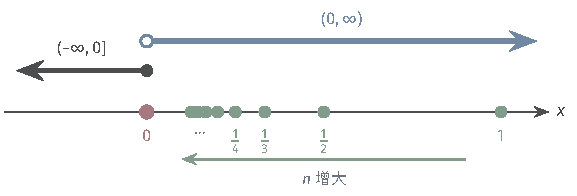
\includegraphics[width=97.6mm]{figures/07-probability/03-probability-limits/tikz/weak-boundary-mass/figure.pdf}
 \caption{质量移到边界上。绿点为$\delta_{1/n}$的质点位置$1,\,1/2,\,1/3,\dots$，红点为极限$\delta_0$的质点。蓝色为开集$(0,\infty)$，深灰为闭集$(-\infty,0]$，二者的公共边界是$0$：每个$\delta_{1/n}$都把全部质量放在开集里，极限却把它放在闭集里。}
 \label{fig:weak-boundary-mass}
\end{BookInlineFigure}

\subsection{Portmanteau定理}
\label{sec:weak-portmanteau}

图~\ref{fig:weak-boundary-mass}还显示了一个方向性：质量从开集一侧移到边界，闭集$(-\infty,0]$在极限中多得了质量，开集$(0,\infty)$在极限中失去了质量。一般地，极限过程中闭集的概率只能“突然增加”，开集的概率只能“突然减少”。用连续函数逼近示性函数，可以把这个直观变成不等式。

闭集$F$的示性函数由式~\eqref{eq:weak-closed-approx}的$f_k$从上方逼近。对开集$G$，补集$G^{\mathrm{c}}$闭，令
\begin{equation}
 g_k(\bm{x})=\min\bigl(1,\,k\operatorname{dist}(\bm{x},G^{\mathrm{c}})\bigr),\qquad k=1,2,\dots .
 \label{eq:weak-open-approx}
\end{equation}
$g_k$连续，取值在$[0,1]$中，在$G^{\mathrm{c}}$上为零，并且逐点不减地趋于$\mathbf{1}_G$：$\bm{x}\in G$时$\operatorname{dist}(\bm{x},G^{\mathrm{c}})>0$，$k$足够大后$g_k(\bm{x})=1$。图~\ref{fig:weak-portmanteau-approx}画出了区间上的这两族函数。

\begin{BookInlineFigure}
 \centering
 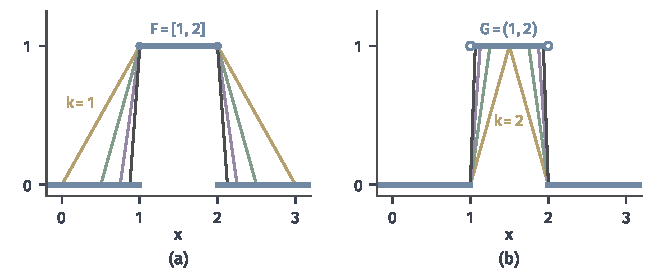
\includegraphics[width=112mm]{figures/07-probability/03-probability-limits/matplotlib/weak-portmanteau-approx/figure.pdf}
 \caption{用连续函数逼近示性函数。(a)闭区间$F=[1,2]$，$f_k$从上方逼近$\mathbf{1}_F$（蓝色粗线），黄、绿、紫、深灰依次为$k=1,2,4,8$。(b)开区间$G=(1,2)$，$g_k$从下方逼近$\mathbf{1}_G$，四种颜色依次为$k=2,4,8,16$。}
 \label{fig:weak-portmanteau-approx}
\end{BookInlineFigure}

\begin{theorem}[Portmanteau定理]
\label{thm:weak-portmanteau}
设$P_n$（$n\geq1$）与$P$是$\mathbb{R}^{d}$上的概率分布。以下五条等价：
\begin{enumerate}
 \item $P_n\xrightarrow{\mathrm{w}}P$；
 \item 对每个有界且Lipschitz连续的$f$，$\int f\,\mathrm{d}P_n\to\int f\,\mathrm{d}P$；
 \item 对每个闭集$F$，$\limsup_{n}P_n(F)\leq P(F)$；
 \item 对每个开集$G$，$\liminf_{n}P_n(G)\geq P(G)$；
 \item 对每个满足$P(\partial A)=0$的Borel集$A$，$P_n(A)\to P(A)$。
\end{enumerate}
\end{theorem}

\begin{proof}
(1)$\Rightarrow$(2)：有界Lipschitz函数是有界连续函数。

(2)$\Rightarrow$(3)：式~\eqref{eq:weak-closed-approx}的$f_k$有界且Lipschitz，并且$f_k\geq\mathbf{1}_F$。固定$k$，
\[
 \limsup_{n\to\infty}P_n(F)\leq\lim_{n\to\infty}\int f_k\,\mathrm{d}P_n=\int f_k\,\mathrm{d}P .
\]
引理~\ref{lem:weak-uniqueness}的证明已经说明$\int f_k\,\mathrm{d}P\to P(F)$。令$k\to\infty$即得(3)。

(3)$\Leftrightarrow$(4)：$G$为开集当且仅当$G^{\mathrm{c}}$为闭集，并且$P_n(G)=1-P_n(G^{\mathrm{c}})$，所以
\[
 \liminf_{n\to\infty}P_n(G)=1-\limsup_{n\to\infty}P_n(G^{\mathrm{c}})\geq1-P(G^{\mathrm{c}})=P(G) .
\]
反方向同理。

(3)与(4)$\Rightarrow$(5)：记$A^{\circ}$为$A$的内部，$\bar{A}$为闭包，则$A^{\circ}\subset A\subset\bar{A}$，且$\bar{A}\setminus A^{\circ}=\partial A$。由$P(\partial A)=0$得$P(A^{\circ})=P(A)=P(\bar{A})$。于是
\[
 \begin{aligned}
 \limsup_{n\to\infty}P_n(A)&\leq\limsup_{n\to\infty}P_n(\bar{A})\leq P(\bar{A})=P(A),\\
 \liminf_{n\to\infty}P_n(A)&\geq\liminf_{n\to\infty}P_n(A^{\circ})\geq P(A^{\circ})=P(A) .
 \end{aligned}
\]
上极限不超过下极限，所以$P_n(A)\to P(A)$。

(5)$\Rightarrow$(1)：取$f\in C_b(\mathbb{R}^{d})$。式~\eqref{eq:weak-definition}两边对$f$都是线性的，常数函数的读数恒为$1$，所以可以对$f$作正的伸缩与平移，不妨设$0<f<1$。由第~\ref{chap:tail-probabilities}章的尾积分公式，
\[
 \int f\,\mathrm{d}P=\int_0^1P(f>t)\,\mathrm{d}t ,
\]
对$P_n$同样成立。

集合$G_t=\{f>t\}$是开集，闭包含于$\{f\geq t\}$，所以$\partial G_t\subset\{f=t\}$。不同$t$对应的集合$\{f=t\}$互不相交，对每个正整数$m$，满足$P(f=t)\geq1/m$的$t$至多$m$个，所以$P(f=t)>0$的$t$至多可数。除去这些$t$，由(5)得$P_n(G_t)\to P(G_t)$。被积函数取值在$[0,1]$中，可数集长度为零，由支配收敛定理，
\[
 \int_0^1P_n(f>t)\,\mathrm{d}t\longrightarrow\int_0^1P(f>t)\,\mathrm{d}t ,
\]
即$\int f\,\mathrm{d}P_n\to\int f\,\mathrm{d}P$。
\end{proof}

\term{Portmanteau定理}（portmanteau theorem）的名字意为“手提箱”，指把几种等价说法装在一起。五条各有用途。(2)把测试函数缩小到有界Lipschitz函数，第~\ref{sec:weak-slutsky}节要用它。(3)和(4)说明极限中闭集可能多得质量、开集可能失去质量，图~\ref{fig:weak-boundary-mass}中两个不等号都是严格的：$\limsup\delta_{1/n}\bigl((-\infty,0]\bigr)=0<1$，$\liminf\delta_{1/n}\bigl((0,\infty)\bigr)=1>0$。(5)给出事件概率真正收敛的条件。

注意(5)中的条件只针对极限分布$P$，不针对$P_n$。格点均匀分布中，$A=[0,1/2]$的边界是$\{0,1/2\}$，$U_n$在$1/2$可能有质量（$n$为偶数时），但$\operatorname{Unif}(0,1)$在边界上没有质量，所以
\[
 \mathbb{P}(U_n\leq1/2)=\frac{\lfloor n/2\rfloor}{n}\longrightarrow\frac12 .
\]
$n=5$时为$0.4$，$n=11$时为$5/11\approx0.4545$，$n=101$时为$50/101\approx0.4950$。

边界有质量时，不能用示性函数代替连续测试函数。$\delta_{1/n}$与$A=(0,\infty)$就是这样：$P(\partial A)=\delta_0(\{0\})=1$，(5)的条件不满足，概率也确实不收敛。

\subsection{分布函数判据}
\label{sec:weak-cdf-criterion}

实轴上的分布由分布函数$F(x)=P\bigl((-\infty,x]\bigr)$确定。事件$(-\infty,x]$的边界是单点$\{x\}$，$P(\{x\})=0$恰好说明$F$在$x$处连续。于是Portmanteau定理的(5)直接给出：弱收敛时，分布函数在极限的连续点处收敛。下面的定理说明反过来也对。

\begin{theorem}[分布函数判据]
\label{thm:weak-cdf-criterion}
设$P_n$与$P$是$\mathbb{R}$上的概率分布，分布函数分别为$F_n$与$F$。则$P_n\xrightarrow{\mathrm{w}}P$，当且仅当
\begin{equation}
 \lim_{n\to\infty}F_n(x)=F(x)\qquad\text{对}F\text{的每个连续点}x .
 \label{eq:weak-cdf-criterion}
\end{equation}
\end{theorem}

\begin{proof}
必要性已由Portmanteau定理的(5)给出。下证充分性，验证(4)。

先说明$F$的连续点在$\mathbb{R}$中稠密。$F$的不连续点是$P$的原子，对每个正整数$m$，质量不小于$1/m$的原子至多$m$个，所以不连续点至多可数。可数集不含任何区间，因此每个区间中都有连续点。把连续点的全体记作$D$。

$\mathbb{R}$中的开集$G$是至多可数个互不相交的开区间之并，记作$G=\bigcup_jI_j$。任取$\varepsilon>0$。由可数可加性，可以取有限个$I_1,\dots,I_m$，使$\sum_{j\leq m}P(I_j)>P(G)-\varepsilon$。

设$I_j=(a_j,b_j)$，端点可以是$\pm\infty$。在$D$中取$a_j<a'_j<b'_j<b_j$，使$a'_j$充分接近$a_j$、$b'_j$充分接近$b_j$。由概率的连续性，可以做到
\[
 P\bigl((a'_j,b'_j]\bigr)>P(I_j)-\varepsilon/m .
\]

$(a'_j,b'_j]\subset I_j$，各$I_j$互不相交，所以
\[
 P_n(G)\geq\sum_{j=1}^{m}P_n\bigl((a'_j,b'_j]\bigr)=\sum_{j=1}^{m}\bigl(F_n(b'_j)-F_n(a'_j)\bigr) .
\]
右边是有限和，由式~\eqref{eq:weak-cdf-criterion}，它趋于
\[
 \sum_{j=1}^{m}\bigl(F(b'_j)-F(a'_j)\bigr)=\sum_{j=1}^{m}P\bigl((a'_j,b'_j]\bigr)>P(G)-2\varepsilon .
\]
于是$\liminf_nP_n(G)\geq P(G)-2\varepsilon$，$\varepsilon$任意，(4)成立。
\end{proof}

为什么必须排除跳点？$\delta_{1/n}$的分布函数是$F_n(x)=\mathbf{1}_{\{x\geq1/n\}}$，极限$\delta_0$的分布函数是$F(x)=\mathbf{1}_{\{x\geq0\}}$。逐点看：
\[
 \begin{aligned}
 &x<0: && F_n(x)=0=F(x);\\
 &x>0: && n>1/x\text{时}F_n(x)=1=F(x);\\
 &x=0: && F_n(0)=0\neq1=F(0) .
 \end{aligned}
\]
只有跳点$0$处不收敛。若质点从左边逼近，即$\delta_{-1/n}$，则$F_n(0)=1\to F(0)$。可见跳点处是否收敛取决于质量从哪一侧靠近，而弱收敛并不区分这两种靠近方式，图~\ref{fig:weak-cdf-criterion}(a)显示了这两种情形。

格点均匀分布的分布函数是阶梯$F_n(x)=\lfloor nx\rfloor/n$（$0\leq x\leq1$），极限$F(x)=x$处处连续。由$nx-1<\lfloor nx\rfloor\leq nx$，
\[
 \sup_{x\in\mathbb{R}}\lvert F_n(x)-F(x)\rvert\leq\frac1n .
\]
这里的收敛还是一致的，见图~\ref{fig:weak-cdf-criterion}(b)。

\begin{BookInlineFigure}
 \centering
 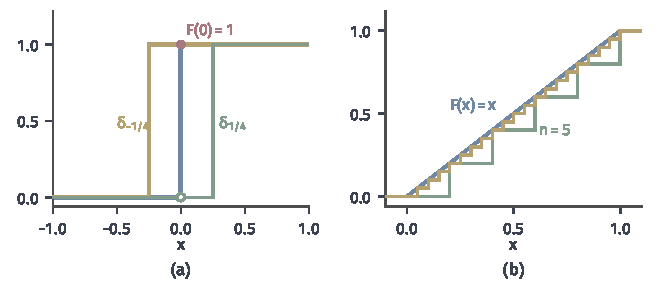
\includegraphics[width=112mm]{figures/07-probability/03-probability-limits/matplotlib/weak-cdf-criterion/figure.pdf}
 \caption{分布函数判据中的跳点。(a)蓝色为$\delta_0$的分布函数，绿色为$\delta_{1/4}$，黄色为$\delta_{-1/4}$；红点为$F(0)=1$，$\delta_{1/n}$在$0$处的值恒为$0$。(b)格点均匀分布$U_5$（绿色阶梯）与$U_{20}$（黄色阶梯）的分布函数，蓝线为$F(x)=x$。}
 \label{fig:weak-cdf-criterion}
\end{BookInlineFigure}

\paragraph{二项分布到Poisson分布}
现在可以把章首的现象写成定理。设$X_n\sim\operatorname{Bin}(n,2/n)$（$n\geq3$），$N\sim\operatorname{Poisson}(2)$。第~\ref{chap:common-distributions}章已经证明，对每个非负整数$k$，$\mathbb{P}(X_n=k)\to\mathbb{P}(N=k)$。分布函数在$x<0$时都为零；$x\geq0$时是有限和
\[
 F_n(x)=\sum_{k=0}^{\lfloor x\rfloor}\mathbb{P}(X_n=k)\longrightarrow\sum_{k=0}^{\lfloor x\rfloor}\mathbb{P}(N=k)=F(x) .
\]
所以$F_n(x)\to F(x)$对每个$x$成立，由定理~\ref{thm:weak-cdf-criterion}，$X_n\xrightarrow{\mathrm{d}}\operatorname{Poisson}(2)$。这里在跳点处也收敛；定理只是允许跳点处不收敛，并不要求它不收敛。

以$x=2$为例，$F(2)=5\mathrm{e}^{-2}\approx0.6767$，而
\[
 F_4(2)=0.6875,\qquad F_{10}(2)=0.6778,\qquad F_{40}(2)=0.6767 .
\]
图~\ref{fig:weak-binomial-poisson}(a)比较两个分布函数，(b)画出$\sup_x\lvert F_n(x)-F(x)\rvert$随$n$的变化，它大致按$1/n$缩小。弱收敛本身只断言极限，不给速度；这个速度是此例的具体计算结果。

\begin{BookInlineFigure}
 \centering
 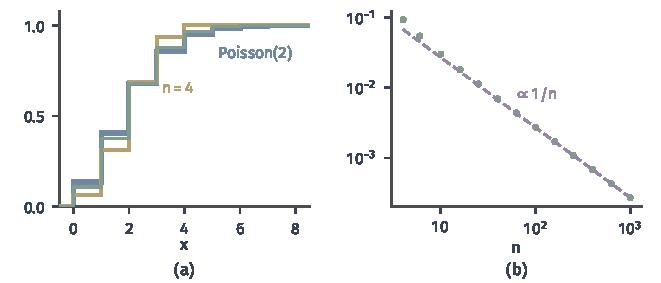
\includegraphics[width=112mm]{figures/07-probability/03-probability-limits/matplotlib/weak-binomial-poisson/figure.pdf}
 \caption{$\operatorname{Bin}(n,2/n)$向$\operatorname{Poisson}(2)$的弱收敛。(a)蓝色阶梯为$\operatorname{Poisson}(2)$的分布函数，黄色为$n=4$，绿色为$n=10$。(b)$\sup_x\lvert F_n(x)-F(x)\rvert$（绿点，对数坐标），紫色虚线是斜率为$-1$的参考线。}
 \label{fig:weak-binomial-poisson}
\end{BookInlineFigure}

分布函数判据还要求极限$F$本身是分布函数。若只知道$F_n$逐点收敛，极限可能不是分布函数：$\delta_n$的分布函数$\mathbf{1}_{\{x\geq n\}}$对每个$x$都趋于$0$。质量逃到了无穷远，下一节研究怎样防止这种情形。
